\problemname{Infinite Race}

Every year, there is a marathon in Eindhoven. This year, the organizers have come up with something special, and instead of being over after 42 kilometres, the race goes on forever!
To keep the organization simple, the race takes place on a running track at Eindhoven university, and the participants run an infinite number of laps on the track.

Anika is excited to be one of the $N$ participants, numbered from $0$ to $N-1$. She was quick to sign up which means she is participant $0$. She starts right after the finish line with all other participants positioned ahead of her on the track. Anika cannot keep track of how many laps she has run, but she remembers when she overtakes someone or when someone overtakes her. What is the minimum number of times she must have crossed the finish line? Nobody moves backwards, and no overtaking happens exactly at the finish line. Furthermore, note that the participants do not necessarily run at a constant speed.

\begin{figure}[h]
    \center
    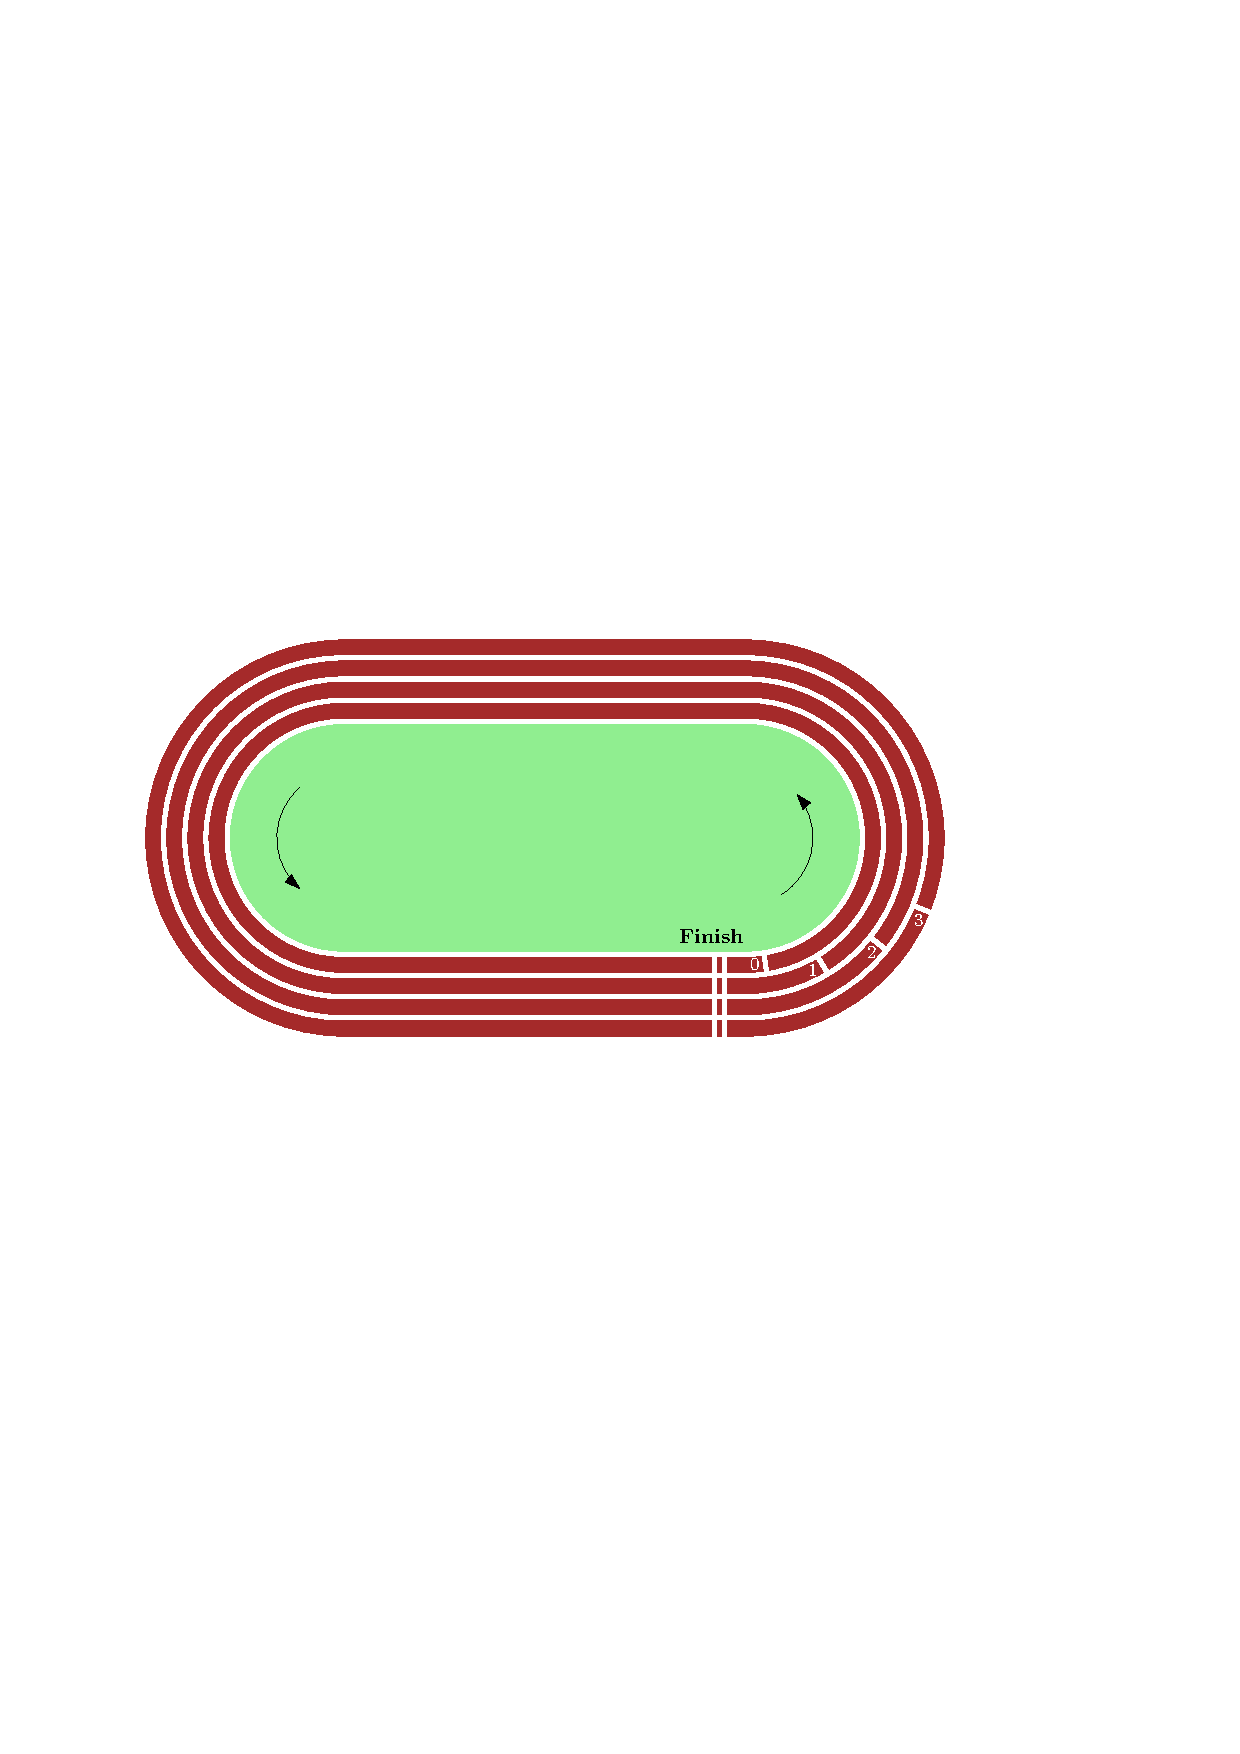
\includegraphics[width=0.7\textwidth]{track}
    \caption{The starting position of the race with $N = 4$ participants.}
\end{figure}

\section*{Input}
The first line of input contains an integer $N$, the number of participants.

The second line contains an integer $Q$, the number of events.

The following $Q$ lines describe the events in the order they occurred during the race.
The $i$th line contains an integer $x_i$.
\begin{itemize}
\item If $x_i > 0$, it means that Anika overtook participant $x_i$.
\item If $x_i < 0$, it means that participant $-x_i$ overtook Anika.
\end{itemize}

\section*{Output}
Output a single integer, the minimum number of times Anika must have crossed the finish line.

\section*{Constraints and Scoring}
\begin{itemize}
\item $2 \le N \le 200\,000$.
\item $1 \le Q \le 200\,000$.
\item $1 \le x_i \le N-1$ or $-(N-1) \le x_i \le -1$.
\end{itemize}


Your solution will be tested on a set of test groups, each worth a number of points.
Each test group contains a set of test cases. To get the points for a test group, you need to solve all test cases in the test group.



\begin{tabular}{|l|l|l|}
\hline
Group  &  Score  &  Limits \\
\hline
 1 & 29 & $N = 2$   \\
\hline
 2 & 34 & $x_{i} > 0$ for all $i$ (that is, Anika only overtakes) \\
\hline
 3 & 22 & $N,Q\leq 100$  \\
\hline
 4 & 15 & No additional constraints \\
\hline
\end{tabular}
\section*{Examples}
Note that some of the samples are not valid input for all test groups.

In the first sample, there are $N = 4$ participants and $Q = 5$ events.
Anika first gets overtaken by $2$, who is now a full lap ahead of her. Then she overtakes $2$ back, followed by overtaking $1$ and then being overtaken by $3$. At this point, Anika can still be on her first lap.  Finally, she overtakes $2$ again, and to do so means that she must have crossed the finish line at least once.

In the second sample, there is just one participant other than Anika. Anika overtakes the other participant four times, meaning that Anika must have crossed the finish line at least three times.
